\section{Overview of the Problem}
Early childhood education (ECE) is crucial in New Zealand, especially for children from disadvantages backgrounds, as it sets them up for better academic and social development. According to a previous research study in New Zealand, children who participate in early learning programs tend to excel academically and socially throughout their schooling \cite{educationcounts}

However, the high cost of childcare in New Zealand, often forces mothers to leave their jobs or seek unconventional childcare solutions, hindering their ability to participate in the workforce. \cite{accesstochildcareinterim} The government's “He Taonga te Tamaiti" | Early Learning Action Plan aims to ensure all children have access to early learning programs \cite{ministryofeducation_2019}. However, despite government 20 hours subsidies, childcare costs in New Zealand remain among the highest globally, exceeding \$300 per week for children over three years old. \cite{stuff_2024} According to figure~\ref{fig:ChildcareCosts}, it shows the cost of New Zealand childcare is among most expensive in the world specially compaired to the other countries in the region. \cite{accesstochildcareinterim}

\begin{figure}[hpt]
	\centering
	{{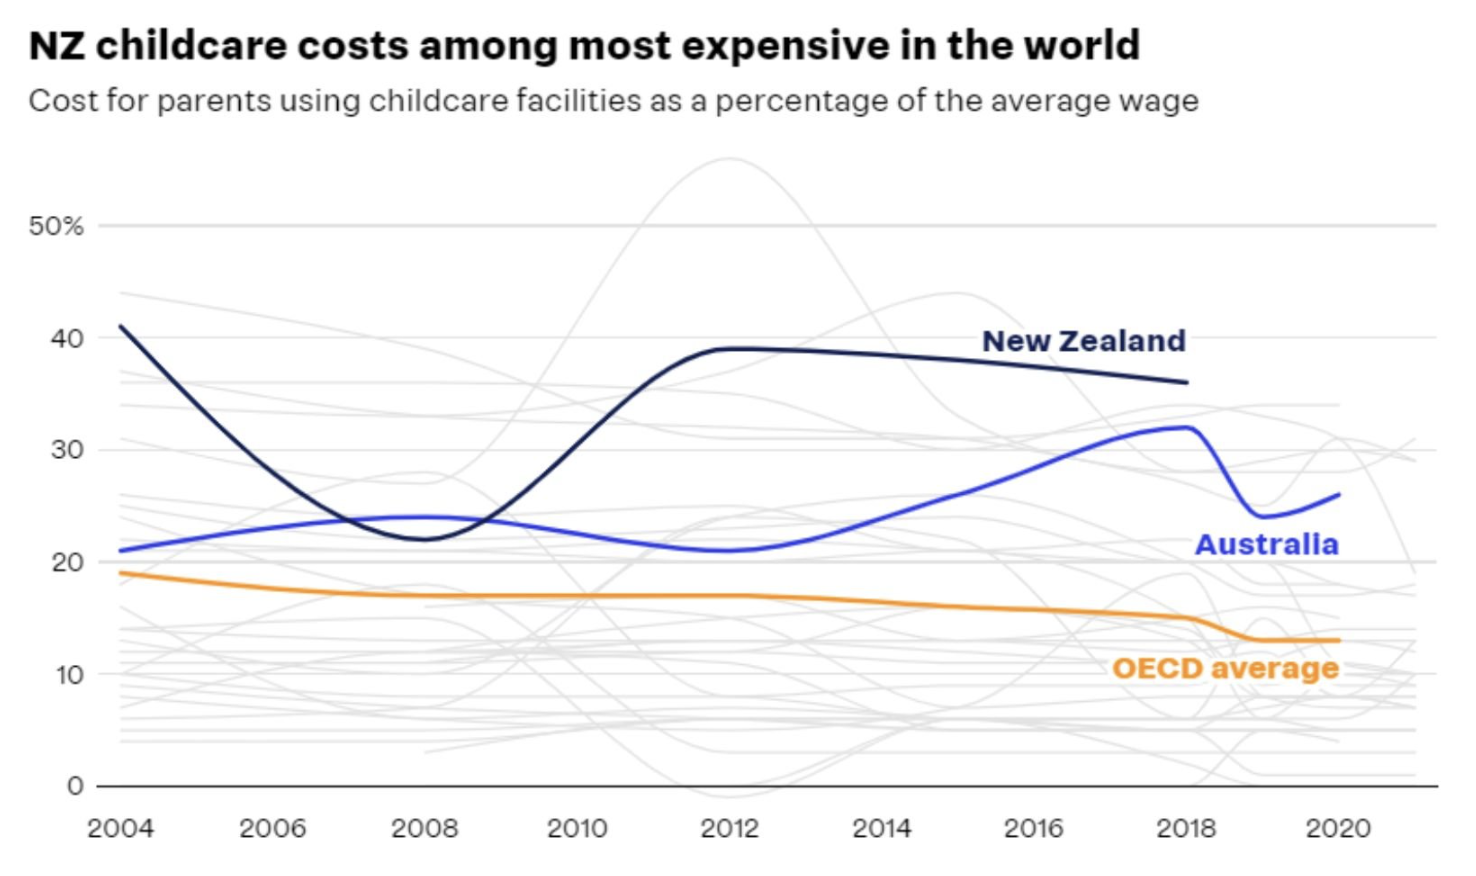
\includegraphics[width=0.9\columnwidth,keepaspectratio]{Figures/figure-1.png} }}
	\caption{NZ childcare costs among most expensive in the world \cite{election_2023}}%
	\label{fig:ChildcareCosts}%
\end{figure}

This financial burden leads many women to make career sacrifices or face difficulties finding affordable and quality childcare options \cite{stuff_2024}. As the figure~\ref{fig:ParticipationDensity} shows from a previous research done in new zealand, it appears that there's a reduced participation intensity of children between age 3-4, beyond the government concession of 20 hour period. \cite{educationcounts_intensity_measure}

\begin{figure}[hpt]
	\centering
	{{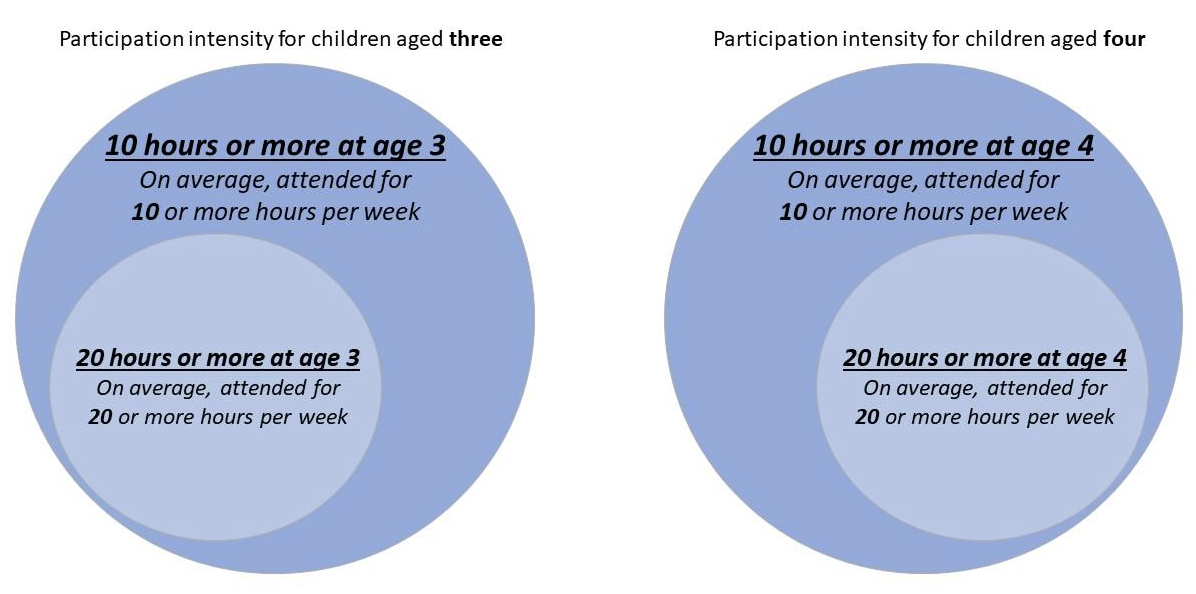
\includegraphics[width=0.9\columnwidth,keepaspectratio]{Figures/figure-2.png} }}
	\caption{Participation intensity grouped by age and the number of hours \cite{educationcounts_intensity_measure}}%
	\label{fig:ParticipationDensity}%
\end{figure}

It further shows that the childcare centers in New Zealand mostly operate independently, each with their own websites and communication channels. This decentralized setup causes inefficiencies for parents, experience teachers, especially new immigrants, who will require to individually contact multiple centers to inquire about availability, suitability and employment oppotunities. This fragmented system inconveniences for both parents and potential employees while posing challenges for childcare centers in reaching more potential clients and enrollment processes.